\documentclass[aspectratio=169, 10pt]{beamer}

% --- Font & Engine Setup ---
\usepackage{iftex}
\ifXeTeX
  \usepackage{fontspec}
  \setsansfont{Arial}[
    BoldFont = Arial Bold,
    ItalicFont = Arial Italic,
    BoldItalicFont = Arial Bold Italic
  ]
  \setmainfont{Arial}
\else
  \usepackage[utf8]{inputenc}
  \usepackage[vietnamese]{babel}
  \usepackage[T5]{fontenc}
  \usepackage{tgheros}
  \renewcommand*\familydefault{\sfdefault}
\fi

% --- Core Packages ---
\usepackage{graphicx}
\usepackage{booktabs}
\usepackage{tikz}
\usepackage{tcolorbox}
\tcbuselibrary{skins}
\usepackage{amsmath, amssymb}
\usepackage{colortbl}

% --- Theme & Navigation ---
\usetheme{default}
\usefonttheme{professionalfonts}
\setbeamertemplate{navigation symbols}{}

% --- Color Palette ---
\definecolor{HUSTRed}{RGB}{183, 28, 28}
\definecolor{MarioBlue}{RGB}{21, 101, 192}
\definecolor{MarioGreen}{RGB}{46, 125, 50}
\definecolor{MarioGold}{RGB}{245, 127, 23}
\definecolor{DarkSlate}{RGB}{33, 43, 54}
\definecolor{CardBg}{RGB}{249, 250, 252}
\definecolor{BorderGray}{RGB}{222, 226, 233}
\definecolor{RowAltBg}{RGB}{242, 245, 249}

% --- Beamer Colors ---
\setbeamercolor{frametitle}{fg=white, bg=HUSTRed}
\setbeamercolor{title}{fg=white, bg=HUSTRed}
\setbeamercolor{item}{fg=HUSTRed}
\setbeamercolor{subitem}{fg=MarioBlue}

% --- Frame Title ---
\setbeamertemplate{frametitle}{%
    \nointerlineskip%
    \begin{beamercolorbox}[wd=\paperwidth, ht=0.90cm, dp=0.18cm, leftskip=0.55cm, rightskip=0.55cm]{frametitle}%
        {\normalsize\textbf{\insertframetitle}}%
        \ifx\insertframesubtitle\@empty\else%
            \ \ \textcolor{MarioGold!50}{|}\ \ {\scriptsize\textmd{\insertframesubtitle}}%
        \fi%
    \end{beamercolorbox}%
    \nointerlineskip%
    {\color{MarioGold}\hrule height 1.3pt}%
}

% --- Footline ---
\setbeamertemplate{footline}{%
    \leavevmode%
    {\color{BorderGray}\hrule height 0.4pt}%
    \hbox{%
        \begin{beamercolorbox}[wd=.38\paperwidth, ht=2.2ex, dp=0.7ex, leftskip=0.5cm]{author in head/foot}%
            \tiny\textcolor{gray}{\textbf{MI4090} (Nhóm 36) -- Khoa Toán Tin (HUST)}%
        \end{beamercolorbox}%
        \begin{beamercolorbox}[wd=.38\paperwidth, ht=2.2ex, dp=0.7ex, center]{title in head/foot}%
            \tiny\textcolor{gray}{Super Mario Bros 2D -- Clean Architecture}%
        \end{beamercolorbox}%
        \begin{beamercolorbox}[wd=.24\paperwidth, ht=2.2ex, dp=0.7ex, rightskip=0.5cm]{date in head/foot}%
            \tiny\hfill \textcolor{gray}{Trang \textbf{\insertframenumber} / \inserttotalframenumber}%
        \end{beamercolorbox}%
    }%
    \vskip0pt%
}

% --- Styled Cards ---
\tcbset{
    enhanced,
    sharp corners,
    boxrule=0.65pt,
    left=5pt, right=5pt, top=3pt, bottom=3pt,
    fonttitle=\bfseries\footnotesize
}

\newtcolorbox{infoCard}[2][]{
    colback=CardBg,
    colframe=MarioBlue,
    title=#2,
    #1
}

\newtcolorbox{coreCard}[2][]{
    colback=CardBg,
    colframe=HUSTRed,
    title=#2,
    #1
}

\newtcolorbox{successCard}[2][]{
    colback=CardBg,
    colframe=MarioGreen,
    title=#2,
    #1
}

\newcommand{\badge}[2]{%
    \colorbox{#1}{\textcolor{white}{\textbf{\scriptsize\,#2\,}}}%
}

\begin{document}

% ==============================================================================
% SLIDE 1: TRANG TIÊU ĐỀ & THÔNG TIN NHÓM
% ==============================================================================
\begin{frame}[plain]
    \begin{tikzpicture}[remember picture, overlay]
        \fill[HUSTRed] (current page.north west) rectangle ([yshift=-2.35cm]current page.north east);
        \fill[MarioGold] ([yshift=-2.35cm]current page.north west) rectangle ([yshift=-2.40cm]current page.north east);

        \node[anchor=north west, text=white] at ([xshift=0.75cm, yshift=-0.35cm]current page.north west) {
            \parbox{14.5cm}{
                \tiny \textbf{TRƯỜNG ĐẠI HỌC BÁCH KHOA HÀ NỘI -- KHOA TOÁN TIN} \\
                \scriptsize BÁO CÁO BÀI TẬP LỚN HỌC PHẦN: LẬP TRÌNH HƯỚNG ĐỐI TƯỢNG (MI4090) -- \textbf{NHÓM 36}
            }
        };
        \node[anchor=north west, text=white] at ([xshift=0.75cm, yshift=-1.10cm]current page.north west) {
            \parbox{14.5cm}{
                \Large \textbf{SUPER MARIO BROS CLONE 2D} \\
                \small \textcolor{MarioGold}{\textbf{Clean Architecture \& GoF Design Patterns Edition}}
            }
        };
    \end{tikzpicture}

    \vspace{2.05cm}
    \begin{columns}[c]
        \begin{column}{0.49\textwidth}
            \begin{coreCard}{Thông tin Đề tài \& Nhóm Thực hiện}
                \begin{itemize}\scriptsize\setlength{\itemsep}{2.5pt}
                    \item \textbf{Đề tài:} Super Mario Bros Clone 2D
                    \item \textbf{Kiến trúc:} Clean Architecture 3 tầng \& GoF Patterns
                    \item \textbf{Học phần:} Lập trình Hướng đối tượng (MI4090)
                    \item \textbf{Đơn vị:} Khoa Toán Tin
                    \item \textbf{Nhóm sinh viên:} \textbf{Nhóm 36}
                    \begin{itemize}\scriptsize
                        \item Đỗ Đình Sinh
                        \item Hoàng Anh Quân
                    \end{itemize}
                    \item \textbf{Mục tiêu:} Tái hiện gameplay kinh điển bám sát chuẩn Clean Code \& Kiểm thử tự động (Unit Test AAA).
                \end{itemize}
            \end{coreCard}
        \end{column}

        \begin{column}{0.48\textwidth}
            \centering
            \begin{tcolorbox}[colback=white, colframe=BorderGray, boxrule=0.8pt, width=\textwidth, top=2pt, bottom=2pt, left=2pt, right=2pt,
                title=\textbf{\scriptsize Giao diện Khởi động (Start Game)}, coltitle=white, colbacktitle=DarkSlate]
                \centering
                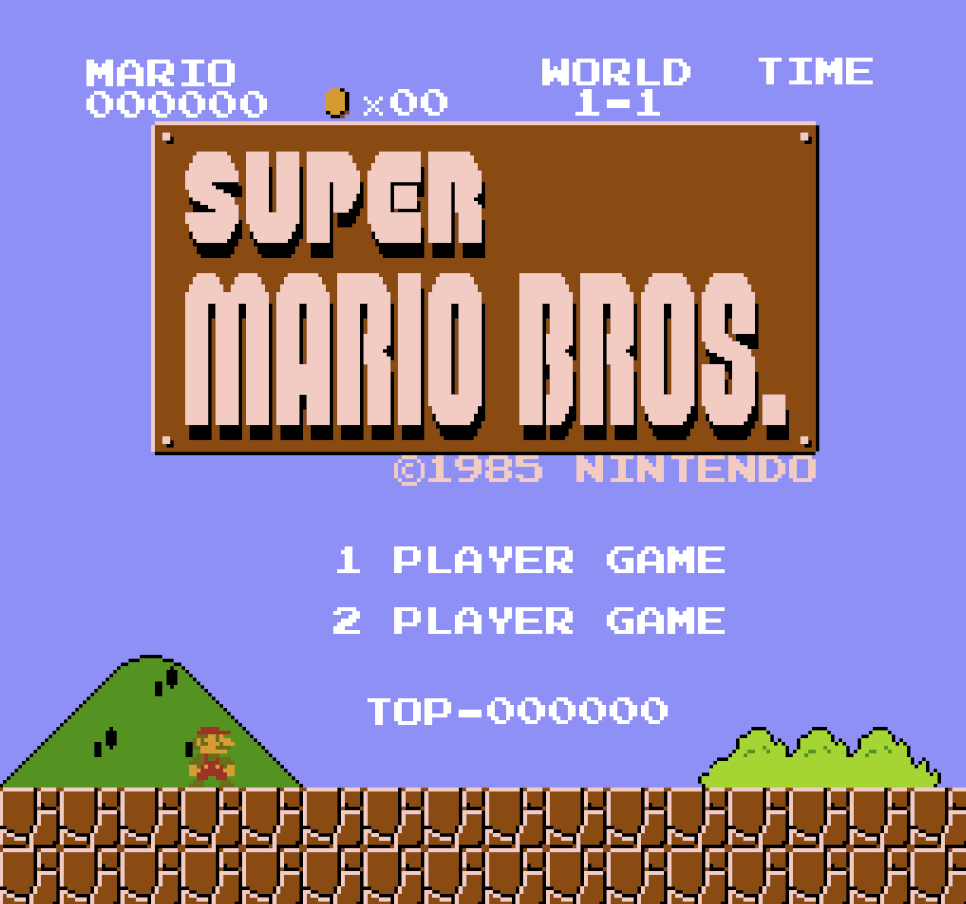
\includegraphics[width=\textwidth, height=4.3cm, keepaspectratio]{assets/start_game.png}
                \\[1pt]
                \tiny \textbf{Hình 1:} Giao diện khởi động Super Mario Bros 2D
            \end{tcolorbox}
        \end{column}
    \end{columns}
\end{frame}

% ==============================================================================
% SLIDE 2: ĐẶT VẤN ĐỀ & MỤC TIÊU ĐỒ ÁN
% ==============================================================================
\begin{frame}{Đặt vấn đề \& Mục tiêu Đồ án}
    \begin{columns}[T]
        \begin{column}{0.50\textwidth}
            \begin{infoCard}{1. Đặt vấn đề}
                \begin{itemize}\scriptsize\setlength{\itemsep}{1.8pt}
                    \item Tái hiện trò chơi kinh điển \textit{Super Mario Bros} bằng \textbf{Unity 6 \& C\#}.
                    \item Xóa bỏ hoàn toàn kiến trúc Monolith dính chặt \texttt{MonoBehaviour}, thiếu cơ chế lưu trữ bền vững và không thể Unit Test ngoài Editor.
                \end{itemize}
            \end{infoCard}

            \begin{successCard}{2. Mục tiêu Chuẩn Điểm A (Khung Kiểm định A $\leftrightarrow$ B)}
                \begin{itemize}\scriptsize\setlength{\itemsep}{1.8pt}
                    \item \textbf{Nhất quán 2 chiều A $\leftrightarrow$ B:} Mô hình thiết kế khớp 100\% với Call Stack thực thi.
                    \item \textbf{Kiến trúc 3 Tầng:} \texttt{Game.Core} thuần C\# đạt \textbf{0\% tham chiếu} \texttt{UnityEngine.dll}.
                    \item \textbf{Định mức Nhóm 2 người:} $\ge$ \textbf{7 PCUs} (5 màn + 2 chế độ) và $\ge$ \textbf{8 Use Cases}.
                \end{itemize}
            \end{successCard}
        \end{column}

        \begin{column}{0.47\textwidth}
            \begin{tcolorbox}[colback=white, colframe=BorderGray, boxrule=0.8pt, top=2pt, bottom=2pt, left=2pt, right=2pt]
                \centering
                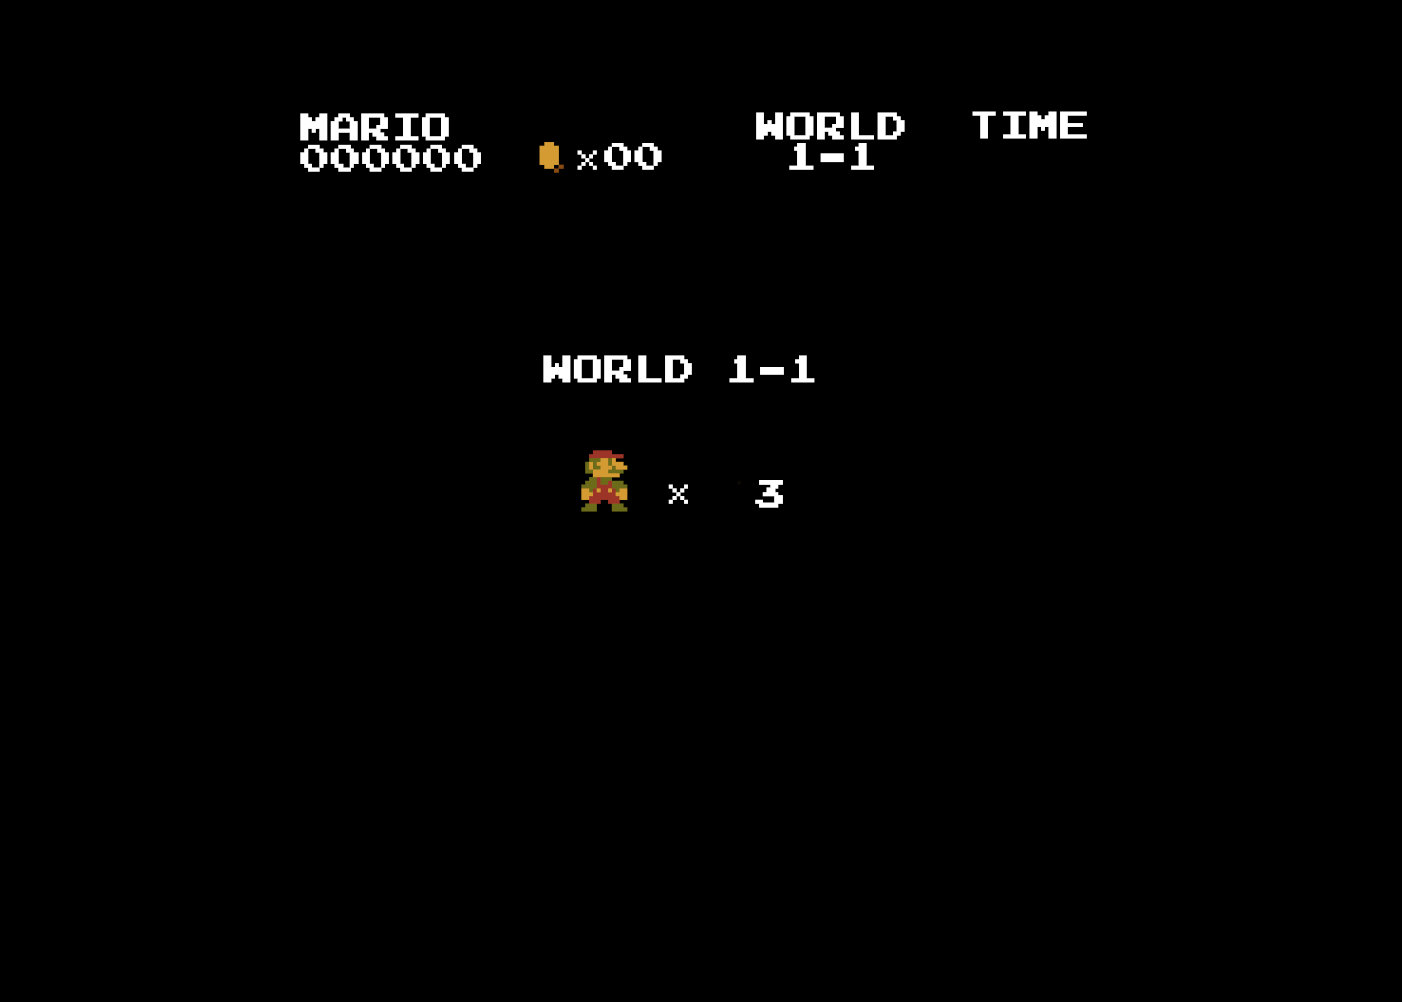
\includegraphics[width=\textwidth, height=4.6cm, keepaspectratio]{assets/life_scene.png}
                \\[1pt]
                \scriptsize \textbf{Hình 2:} Màn hình chuyển cảnh World 1-1
            \end{tcolorbox}
            \vspace{0.05cm}
            \badge{MarioGold}{Tiêu chí Vàng} \scriptsize Clean Architecture + Zero Leakage + Test < 1.0s
        \end{column}
    \end{columns}
\end{frame}

% ==============================================================================
% SLIDE 3: LUẬT CHƠI & CƠ CHẾ TƯƠNG TÁC GAME MARIO
% ==============================================================================
\begin{frame}{Luật chơi \& Cơ chế Tương tác Game Mario}{Quy tắc Màn chơi, Biến hình Power-Up \& Hệ thống Tính điểm}
    \begin{columns}[T]
        \begin{column}{0.50\textwidth}
            \begin{coreCard}[top=2pt, bottom=2pt]{1. Mục tiêu Màn chơi \& Điều kiện Thắng / Thua}
                \begin{itemize}\scriptsize\setlength{\itemsep}{0.8pt}
                    \item \textbf{Mục tiêu:} Điều khiển Mario vượt địa hình, tiêu diệt quái, chạm cờ đích (\texttt{Flagpole}) trước khi hết thời gian (\texttt{Time > 0}).
                    \item \textbf{Thắng:} Chạm cột cờ đích; thời gian dư quy đổi thành điểm thưởng.
                    \item \textbf{Thua:} Rơi xuống vực, hết giờ, hoặc chạm quái khi ở dạng \texttt{Small} $\rightarrow$ Mất 1 mạng (\texttt{Lives - 1}). Hết 3 mạng $\rightarrow$ \texttt{GameOver}.
                \end{itemize}
            \end{coreCard}

            \begin{infoCard}[top=2pt, bottom=2pt]{2. Cơ chế Biến hình \& Chiến đấu}
                \begin{itemize}\scriptsize\setlength{\itemsep}{0.8pt}
                    \item \textbf{Biến hình Power-Up:} \\
                    \centerline{\small $\text{Small Mario} \xrightarrow{+\text{Nấm}} \text{Super} \xrightarrow{+\text{Hoa Lửa}} \text{Fire Mario}$}
                    \item \textbf{Cơ chế Giáp:} Bị sát thương $\rightarrow$ hạ 1 cấp kèm 2s bất tử (\texttt{Invul}).
                    \item \textbf{Tương tác Tiêu diệt:} Giẫm đầu Goomba (+100đ); giẫm Koopa thành mai (+200đ); đá mai rùa dọn quái (+Combo nhân điểm).
                \end{itemize}
            \end{infoCard}
        \end{column}

        \begin{column}{0.47\textwidth}
            \begin{tcolorbox}[colback=white, colframe=BorderGray, boxrule=0.8pt, top=2pt, bottom=2pt, left=2pt, right=2pt]
                \centering
                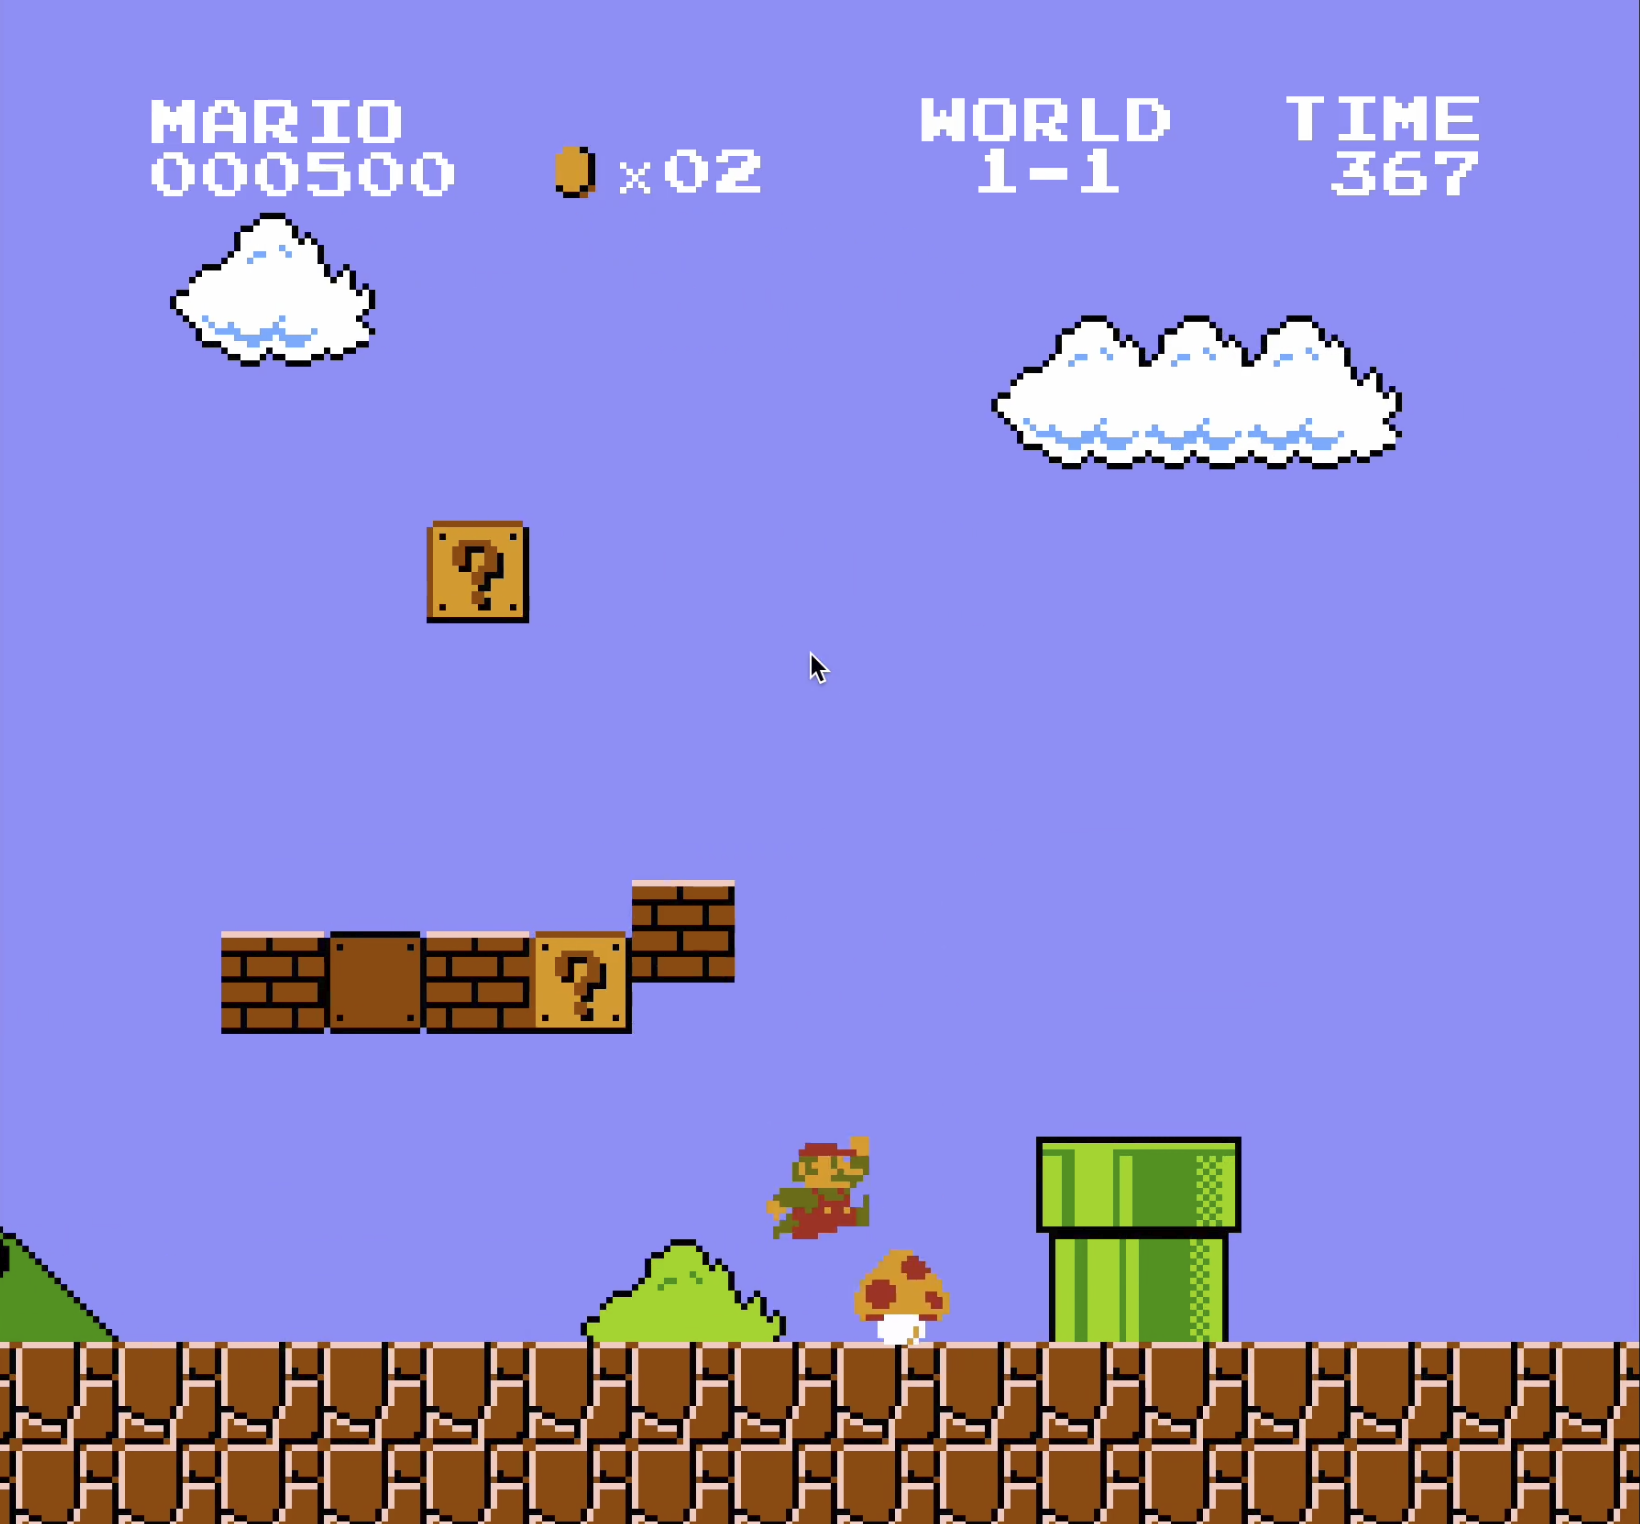
\includegraphics[width=\textwidth, height=4.2cm, keepaspectratio]{assets/in_game_1.png}
                \\[1pt]
                \scriptsize \textbf{Hình 3:} Gameplay World 1-1 với Mario, Khối ? \& Goomba
            \end{tcolorbox}
            \vspace{0.04cm}
            \badge{MarioGold}{Quy tắc Miền} \scriptsize 100 Coin $\rightarrow$ +1 UP; Combo giẫm quái nhân hệ số điểm.
        \end{column}
    \end{columns}
\end{frame}

% ==============================================================================
% SLIDE 4: PHÂN RÃ QUY MÔ MÀN CHƠI & 8 USE CASES
% ==============================================================================
\begin{frame}{Phân rã Quy mô Màn chơi \& Danh mục 8 Use Cases}
    \begin{columns}[T]
        \begin{column}{0.51\textwidth}
            \textbf{\footnotesize \textcolor{HUSTRed}{Danh mục 7 PCUs (5 Màn + 2 Chế độ chơi)}}
            \vspace{0.04cm}
            \begin{table}[h]
                \centering
                \tiny
                \begin{tabular}{@{}llp{3.3cm}@{}}
                    \toprule
                    \textbf{Mã PCU} & \textbf{Tên màn / Chế độ} & \textbf{Đặc trưng cơ chế \& Địa hình} \\
                    \midrule
                    \rowcolor{RowAltBg} PCU-01 & World 1-1 (Grassland) & Đồng cỏ mở, Goomba tuần tra, Khối ? \\
                    PCU-02 & World 1-2 (Underground) & Hầm trần thấp, Koopa dội mai, hố sâu \\
                    \rowcolor{RowAltBg} PCU-03 & World 1-3 (Athletic) & Bật nhảy nền tảng mây, quái truy đuổi \\
                    PCU-04 & World 1-4 (Castle) & Lâu đài dung nham, vòng lửa, Piranha \\
                    \rowcolor{RowAltBg} PCU-05 & Level Select Hub & Danh mục chọn màn chơi nạp từ JSON \\
                    PCU-06 & Classic Mode & Chế độ chơi tiêu chuẩn vượt 4 ải \\
                    \rowcolor{RowAltBg} PCU-07 & Speedrun Boss Arena & Đấu trường Boss Bowser tính giờ \\
                    \bottomrule
                \end{tabular}
            \end{table}

            \vspace{-0.12cm}
            \textbf{\footnotesize \textcolor{MarioBlue}{Phân chia 8 Use Cases Liên phân hệ (Chia đều TV1 -- TV2)}}
            \begin{itemize}\tiny\setlength{\itemsep}{0.8pt}
                \item \textbf{TV1 (Core):} UC01 Init Session; UC03 Movement \& FSM; UC04 AABB Collision; UC07 Save/Load JSON.
                \item \textbf{TV2 (App/Infra):} UC02 Level Select; UC05 Combo Scoring; UC06 Pause \& Cheat; UC08 HighScore Board.
            \end{itemize}
        \end{column}

        \begin{column}{0.46\textwidth}
            \begin{tcolorbox}[colback=white, colframe=BorderGray, boxrule=0.8pt, top=2pt, bottom=2pt, left=2pt, right=2pt]
                \centering
                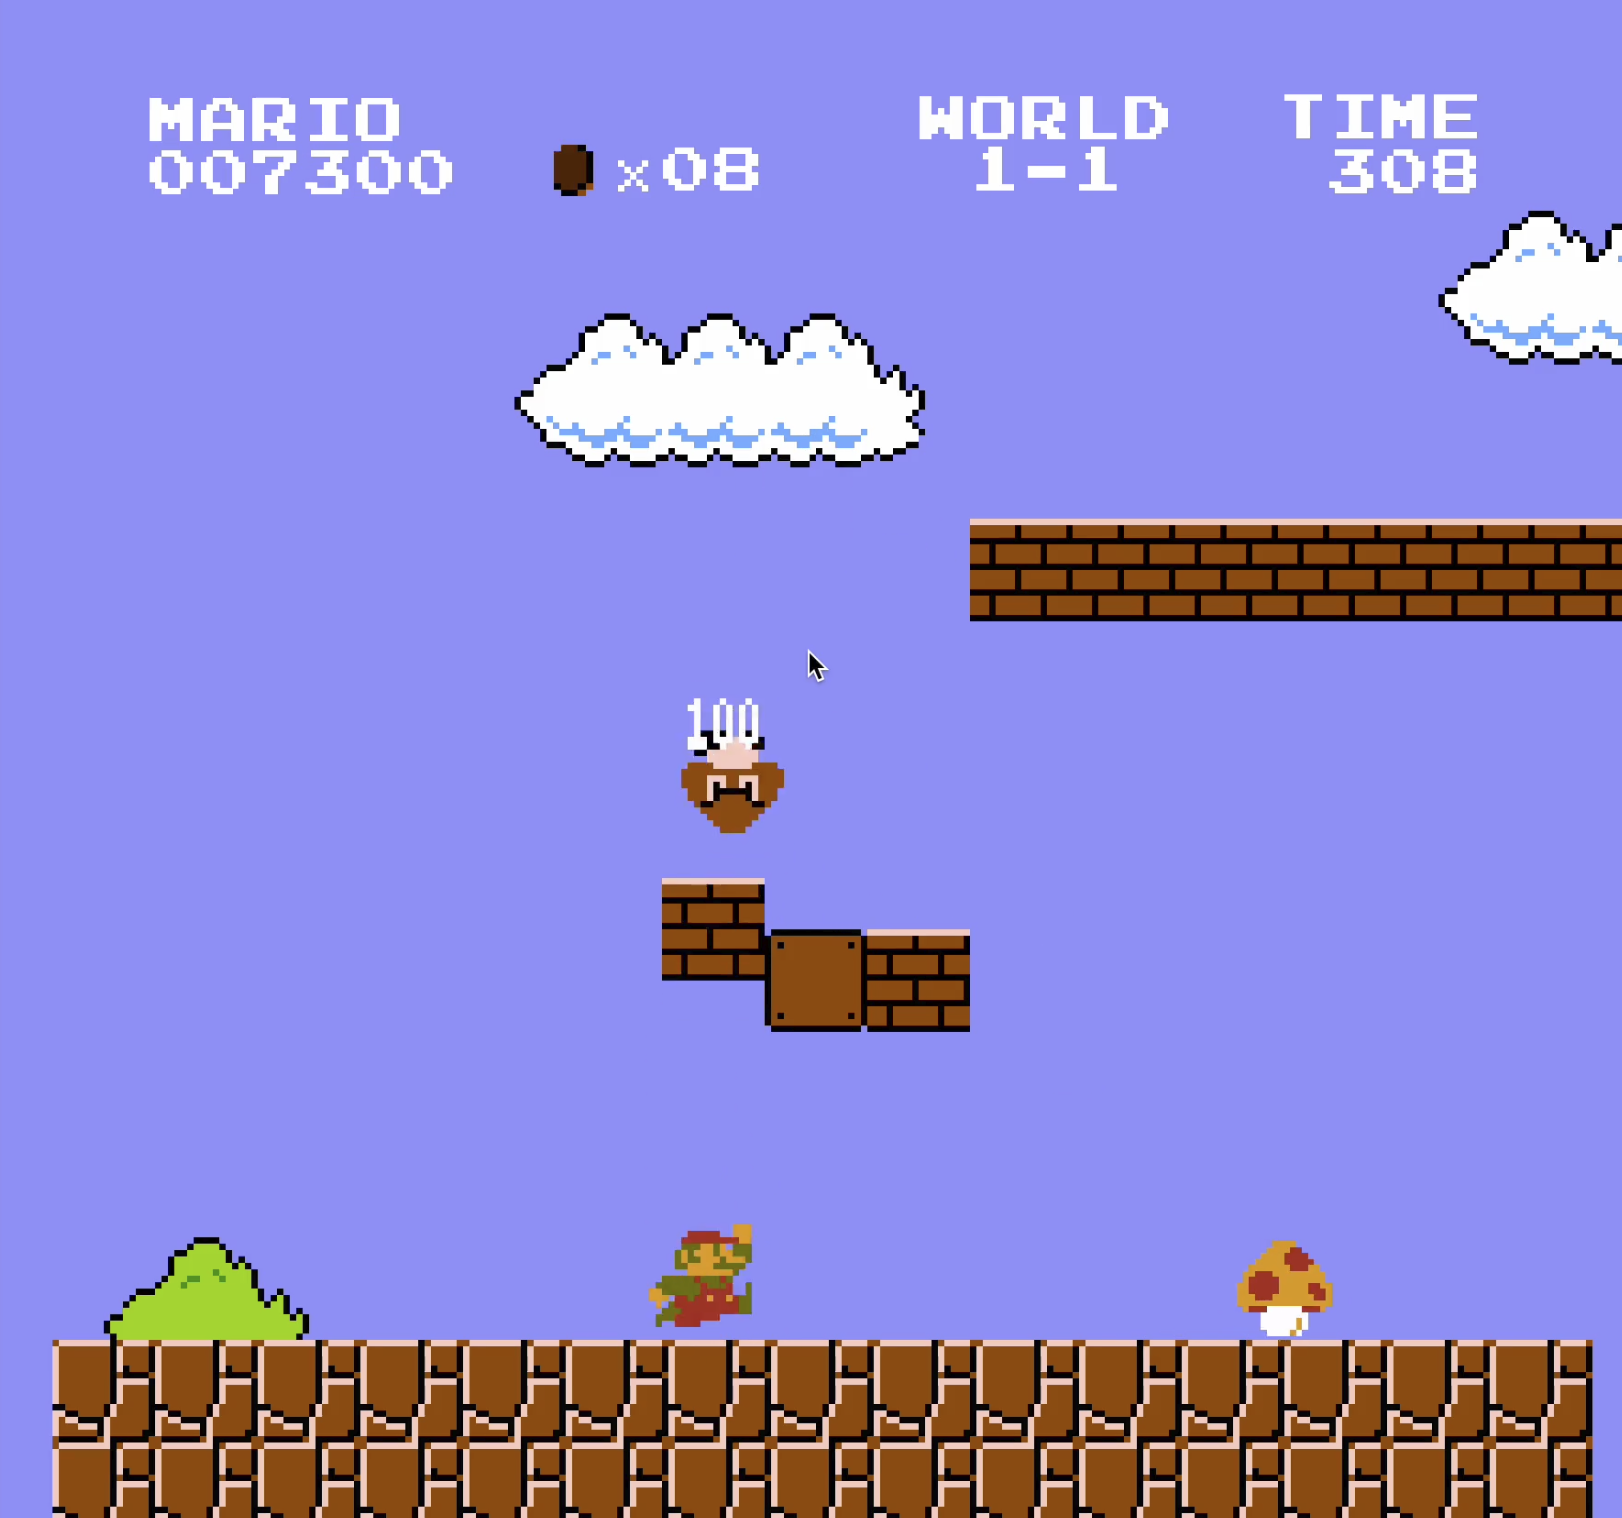
\includegraphics[width=\textwidth, height=4.6cm, keepaspectratio]{assets/in_game_2.png}
                \\[1pt]
                \scriptsize \textbf{Hình 4:} Màn chơi World 1-2 Underground với Koopa \& Hố sâu
            \end{tcolorbox}
            \vspace{0.05cm}
            \badge{MarioGreen}{DoD Pass} \scriptsize Đạt $\ge 7$ PCU và 8 Use Cases liên thông.
        \end{column}
    \end{columns}
\end{frame}

% ==============================================================================
% SLIDE 5: THỰC THỂ GAME & THUỘC TÍNH CỐT LÕI
% ==============================================================================
\begin{frame}{Thực thể Game \& Thuộc tính Cốt lõi}{Mô hình hóa Đối tượng Miền Pure C\# trong Game.Core}
    \begin{columns}[T]
        \begin{column}{0.50\textwidth}
            \begin{coreCard}[top=1pt, bottom=1pt]{1. Thực thể Nhân vật \& Kẻ địch (Living Entities)}
                \begin{itemize}\scriptsize\setlength{\itemsep}{0.2pt}
                    \item \textbf{\texttt{Player}:} \texttt{Position}, \texttt{Velocity}, \texttt{State} (Small/Super/Fire), \texttt{Lives}, \texttt{Score}. \\
                    \textit{Hành vi:} \texttt{Move()}, \texttt{Jump()}, \texttt{TakeDamage()}, \texttt{PowerUp()}, \texttt{ShootFireball()}.
                    \item \textbf{\texttt{Enemy}:} Goomba, Koopa, Bowser -- \texttt{Velocity}, \texttt{Health}, \texttt{State}. \\
                    \textit{Hành vi:} \texttt{UpdateAI()}, \texttt{OnStomped()}, \texttt{ReverseDirection()}.
                \end{itemize}
            \end{coreCard}

            \vspace{-0.18cm}
            \begin{infoCard}[top=1pt, bottom=1pt]{2. Thực thể Môi trường \& Vật phẩm (Items \& Blocks)}
                \begin{itemize}\scriptsize\setlength{\itemsep}{0.2pt}
                    \item \textbf{\texttt{Item}:} Coin, Mushroom, Flower, Star -- \texttt{Type}, \texttt{Velocity}, \texttt{PointValue}. \\
                    \textit{Hành vi:} \texttt{ApplyEffect(Player)} (tăng mạng, biến hình Mario).
                    \item \textbf{\texttt{Block}:} Brick, ?, Pipe -- \texttt{BlockType}, \texttt{Content}, \texttt{IsBreakable}. \\
                    \textit{Hành vi:} \texttt{OnBumped()} (nảy vật phẩm, phá hủy khối gạch).
                \end{itemize}
            \end{infoCard}
        \end{column}

        \begin{column}{0.47\textwidth}
            \begin{tcolorbox}[colback=white, colframe=BorderGray, boxrule=0.8pt, top=2pt, bottom=2pt, left=2pt, right=2pt]
                \centering
                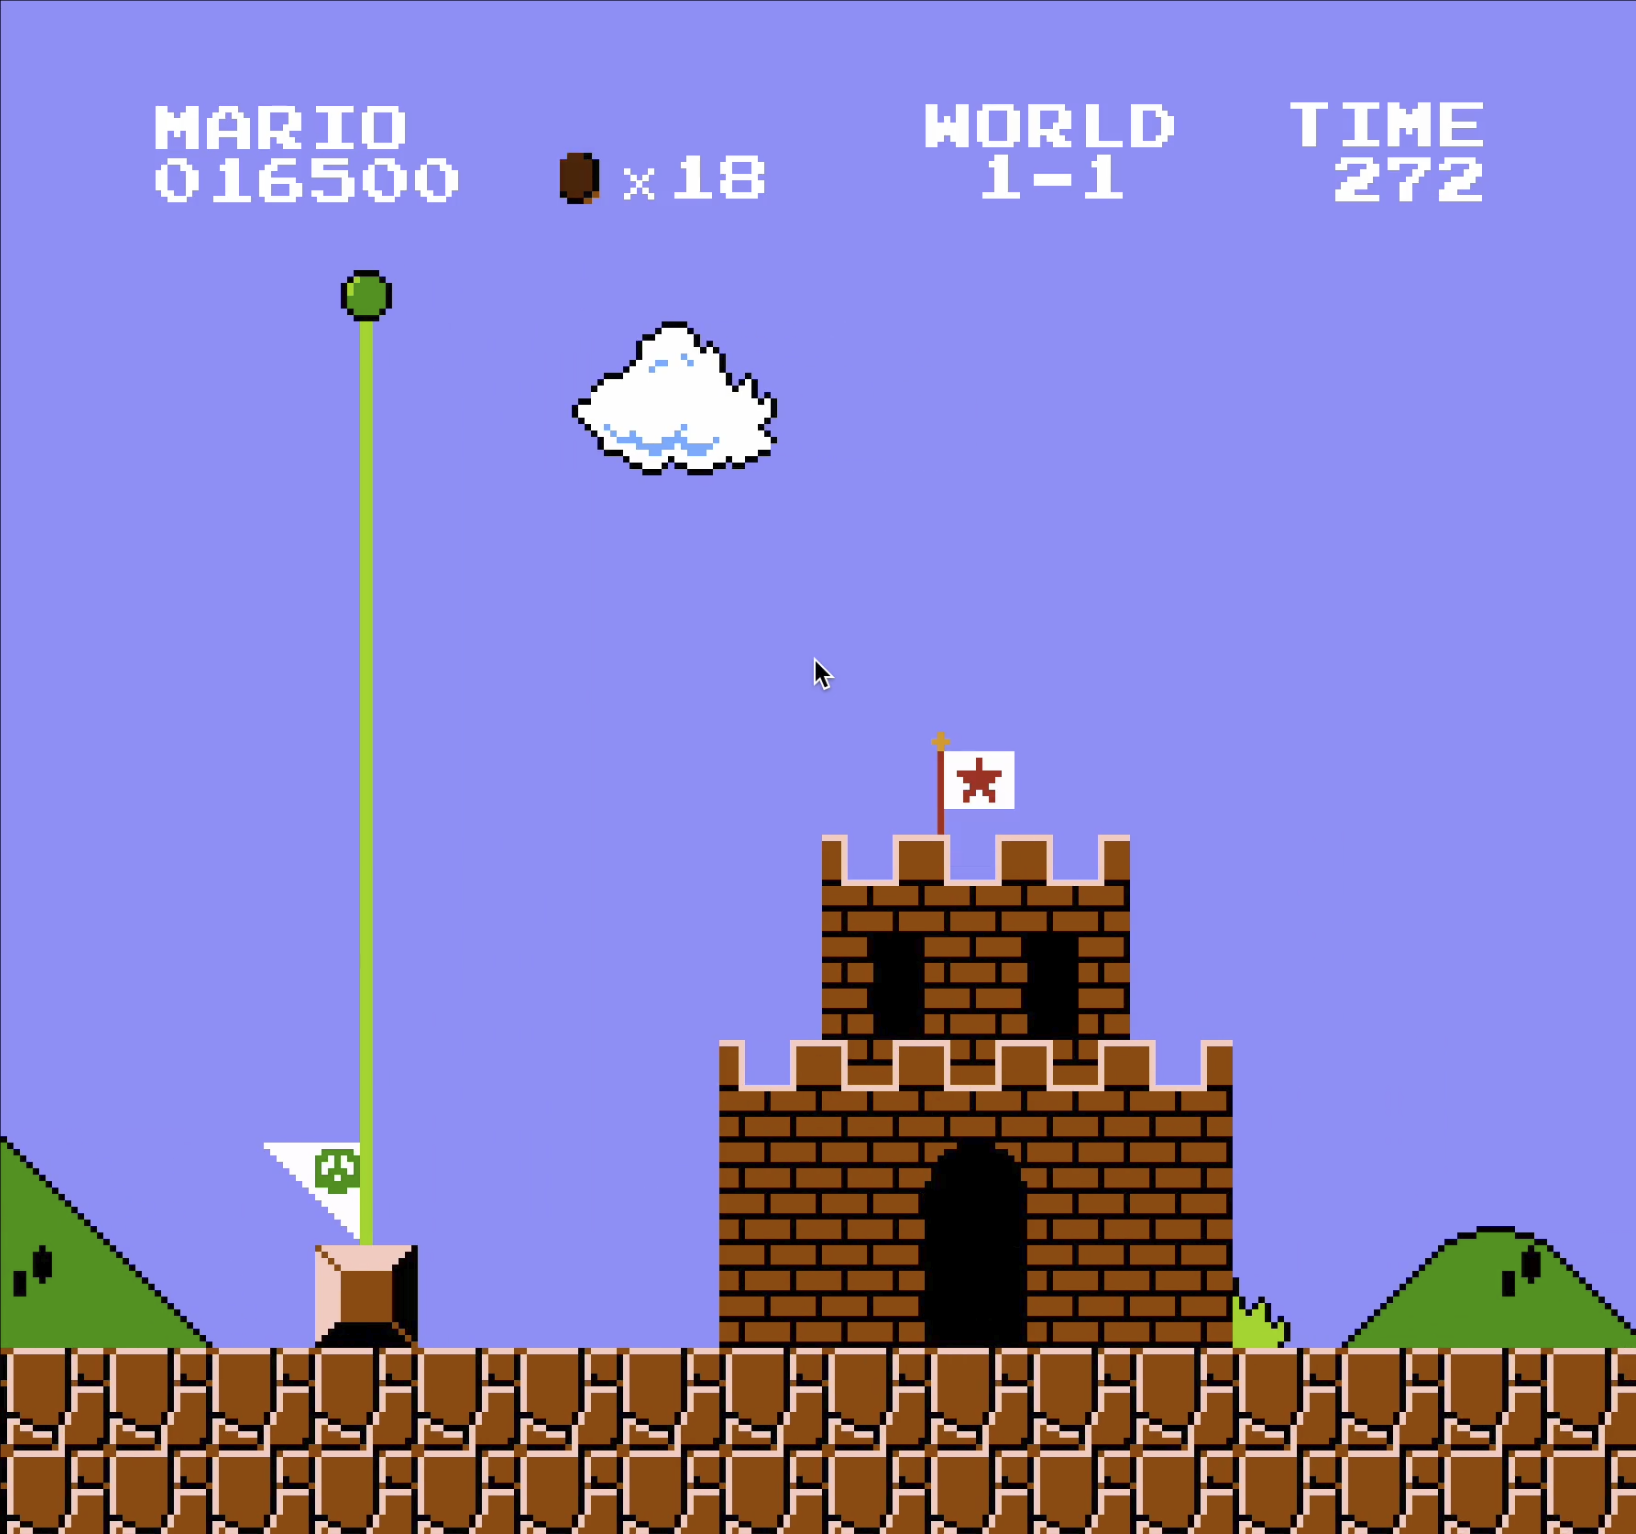
\includegraphics[width=\textwidth, height=3.6cm, keepaspectratio]{assets/in_game_3.png}
                \\[1pt]
                \scriptsize \textbf{Hình 5:} Mario Fire Mario bắn Fireball tiêu diệt Kẻ địch
            \end{tcolorbox}
            \vspace{0.04cm}
            \badge{HUSTRed}{Domain Invariant} \scriptsize Khóa \texttt{private set}, kiểm soát đột biến qua Domain Methods.
        \end{column}
    \end{columns}
\end{frame}

% ==============================================================================
% SLIDE 6: THUẬT TOÁN CỐT LÕI & TRÍ TUỆ NHÂN TẠO (AI)
% ==============================================================================
\begin{frame}{Thuật toán Cốt lõi \& Trí tuệ Nhân tạo (AI)}
    \begin{columns}[T]
        \begin{column}{0.485\textwidth}
            \begin{infoCard}{1. Thuật toán Va chạm Physics AABB \& Sweep Guard}
                \begin{itemize}\scriptsize\setlength{\itemsep}{2pt}
                    \item \textbf{Khoảng chồng lấn 2 trục (Overlap Condition):}
                    $$\Delta x = \min(A.x_2, B.x_2) - \max(A.x_1, B.x_1) > 0$$
                    $$\Delta y = \min(A.y_2, B.y_2) - \max(A.y_1, B.y_1) > 0$$
                    \item \textbf{Penetration Resolution:} Đẩy lùi Mario theo trục nhỏ nhất $\min(\Delta x, \Delta y)$, chống kẹt góc tường (Snag Bug).
                    \item \textbf{Continuous Sweep Raycast:} Tính trước va chạm theo $v \cdot \Delta t$, chống xuyên tường (Tunneling) khi tốc độ cao.
                    \item \textbf{Độ phức tạp:} $O(1)$ mỗi cặp thực thể; $O(N)$ quét phân vùng cục bộ.
                \end{itemize}
            \end{infoCard}
        \end{column}

        \begin{column}{0.485\textwidth}
            \begin{coreCard}{2. Trí tuệ Nhân tạo (AI) \& Hệ thống Dữ liệu}
                \begin{itemize}\scriptsize\setlength{\itemsep}{2pt}
                    \item \textbf{Goomba (1D Patrol AI):} Di chuyển $2.0\,\text{m/s}$; tự đảo chiều $v_x \leftarrow -v_x$ khi gặp vật cản hoặc mép vực (Ledge Detection).
                    \item \textbf{Koopa Troopa (Shell FSM):} State Machine 3 trạng thái:
                    $$\text{Walking} \xrightarrow{\text{Giẫm}} \text{Shell} \xrightarrow{\text{Đá}} \text{MovingShell}\ (12\,\text{m/s})$$
                    \item \textbf{Bowser Boss (Distance AI):} Nhảy dậm đất khi $d \le 4\text{m}$, khạc lửa khi $d > 8\text{m}$, Enrage khi $\text{HP} \le 30\%$.
                    \item \textbf{Save File Integrity:} Ném ngoại lệ \texttt{SaveCorruptedException} khi tệp save bị can thiệp sai cấu trúc.
                \end{itemize}
            \end{coreCard}
        \end{column}
    \end{columns}
\end{frame}

% ==============================================================================
% SLIDE 7: KIẾN TRÚC PHẦN MỀM 3 TẦNG
% ==============================================================================
\begin{frame}{Kiến trúc Phần mềm 3 Tầng (Package Diagram)}
    \begin{columns}[T]
        \begin{column}{0.50\textwidth}
            \begin{coreCard}{\texttt{Game.Core} (Pure C\# Class Library)}
                \begin{itemize}\scriptsize\setlength{\itemsep}{1.2pt}
                    \item \textbf{Domain Entities:} \texttt{Player}, \texttt{Enemy}, \texttt{Item}, \texttt{Block}, \texttt{Vector2D}.
                    \item \textbf{Domain Services:} \texttt{MarioRuleEngine}, \texttt{GameSession}, \texttt{AABBCollisionSystem}.
                    \item \textbf{Ports / Interfaces:} \texttt{IInputProvider}, \texttt{ISaveStorage}, \texttt{IHudObserver}.
                    \item \textbf{Kiểm toán Using:} \textbf{0\%} \texttt{using UnityEngine;}, chạy độc lập hoàn toàn.
                \end{itemize}
            \end{coreCard}

            \begin{infoCard}{\texttt{Game.Infrastructure} \& \texttt{Game.Presentation}}
                \begin{itemize}\scriptsize\setlength{\itemsep}{1.2pt}
                    \item \textbf{Infrastructure:} \texttt{JsonLevelLoader}, \texttt{JsonSaveRepository}, \texttt{ObjectPool<T>}.
                    \item \textbf{Presentation (Unity):} \texttt{MarioView}, \texttt{TilemapRenderer}, \texttt{UnityInputAdapter}.
                \end{itemize}
            \end{infoCard}

            \vspace{0.05cm}
            \badge{HUSTRed}{Kiểm định A $\leftrightarrow$ B} \scriptsize 0 Circular Dependency -- Chạy Headless Tests không mở Unity.
        \end{column}

        \begin{column}{0.47\textwidth}
            \begin{tcolorbox}[colback=white, colframe=BorderGray, boxrule=0.8pt, top=2pt, bottom=2pt, left=2pt, right=2pt]
                \centering
                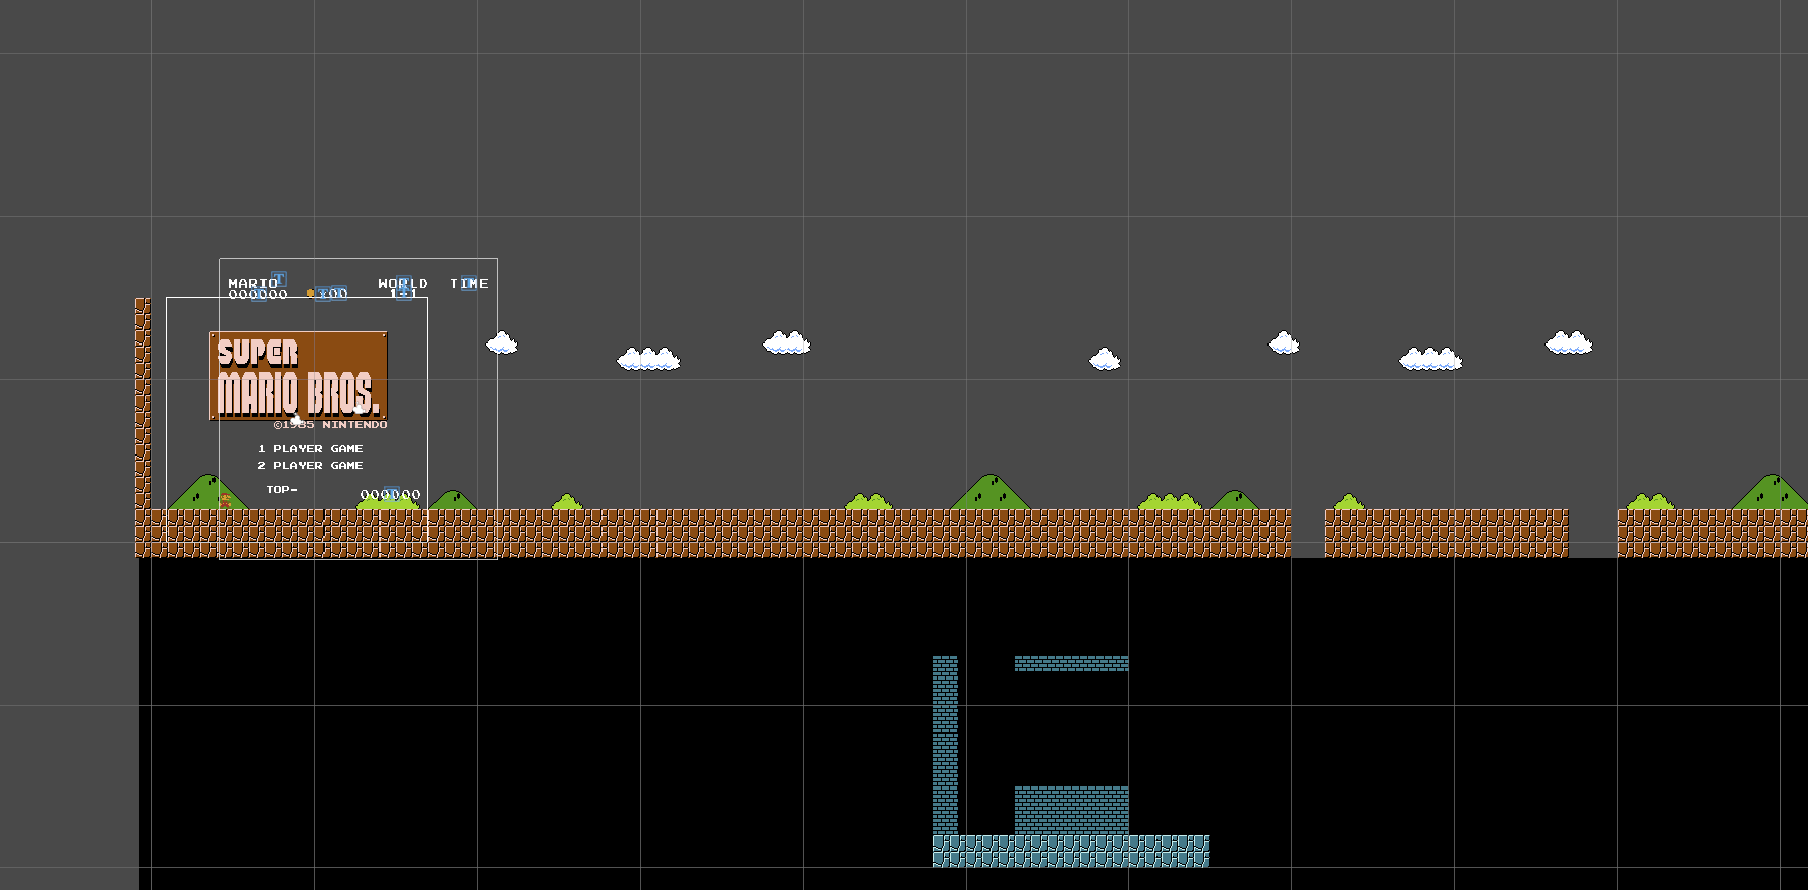
\includegraphics[width=\textwidth, height=4.7cm, keepaspectratio]{assets/edit_1.png}
                \\[1pt]
                \scriptsize \textbf{Hình 6:} Edit bằng UNITY 6.6
            \end{tcolorbox}
        \end{column}
    \end{columns}
\end{frame}

% ==============================================================================
% SLIDE 8: MÔ HÌNH MIỀN & UML CLASS DIAGRAM
% ==============================================================================
\begin{frame}{Mô hình Miền (Domain Model) \& UML Class Diagram}
    \begin{columns}[T]
        \begin{column}{0.50\textwidth}
            \textbf{\footnotesize \textcolor{HUSTRed}{6 Mối quan hệ UML Chuẩn mực trong Mã nguồn:}}
            \begin{itemize}\scriptsize\setlength{\itemsep}{1.2pt}
                \item \textbf{Generalization ($\vartriangle$):} \texttt{CharacterEntity} $\leftarrow$ \texttt{Player}, \texttt{EnemyEntity}.
                \item \textbf{Realization ($\dashrightarrow\vartriangle$):} \texttt{IMarioState} $\leftarrow$ \texttt{SmallState}, \texttt{SuperState}; \texttt{ISaveStorage} $\leftarrow$ \texttt{JsonSaveStorage}.
                \item \textbf{Composition ($\blacklozenge$):} \texttt{GameSession} $\blacklozenge$ \texttt{MarioRuleEngine} (Vòng đời gắn chặt).
                \item \textbf{Aggregation ($\lozenge$):} \texttt{GameSession} $\lozenge$ \texttt{EnemyEntity} (Nhận danh sách từ loader ngoài).
                \item \textbf{Association ($\rightarrow$):} \texttt{Player} $\rightarrow$ \texttt{IMarioState} (Con trỏ trạng thái hiện hành).
                \item \textbf{Dependency ($\dashrightarrow$):} \texttt{MarioRuleEngine} $\dashrightarrow$ \texttt{CollisionResult} (Tham số hàm).
            \end{itemize}

            \begin{successCard}{Bảo vệ Bất biến Miền (Domain Invariants)}
                \begin{itemize}\scriptsize\setlength{\itemsep}{0.8pt}
                    \item \textbf{Encapsulation:} Mạng $0 \le \text{Lives} \le 99$, khóa \texttt{private set}, cập nhật qua \texttt{LoseLife()}.
                    \item \textbf{Read-Only Exposure:} \texttt{IReadOnlyList<EnemyEntity>} ngăn UI can thiệp thực thể.
                \end{itemize}
            \end{successCard}
        \end{column}

        \begin{column}{0.47\textwidth}
            \begin{tcolorbox}[colback=white, colframe=BorderGray, boxrule=0.8pt, top=2pt, bottom=2pt, left=2pt, right=2pt]
                \centering
                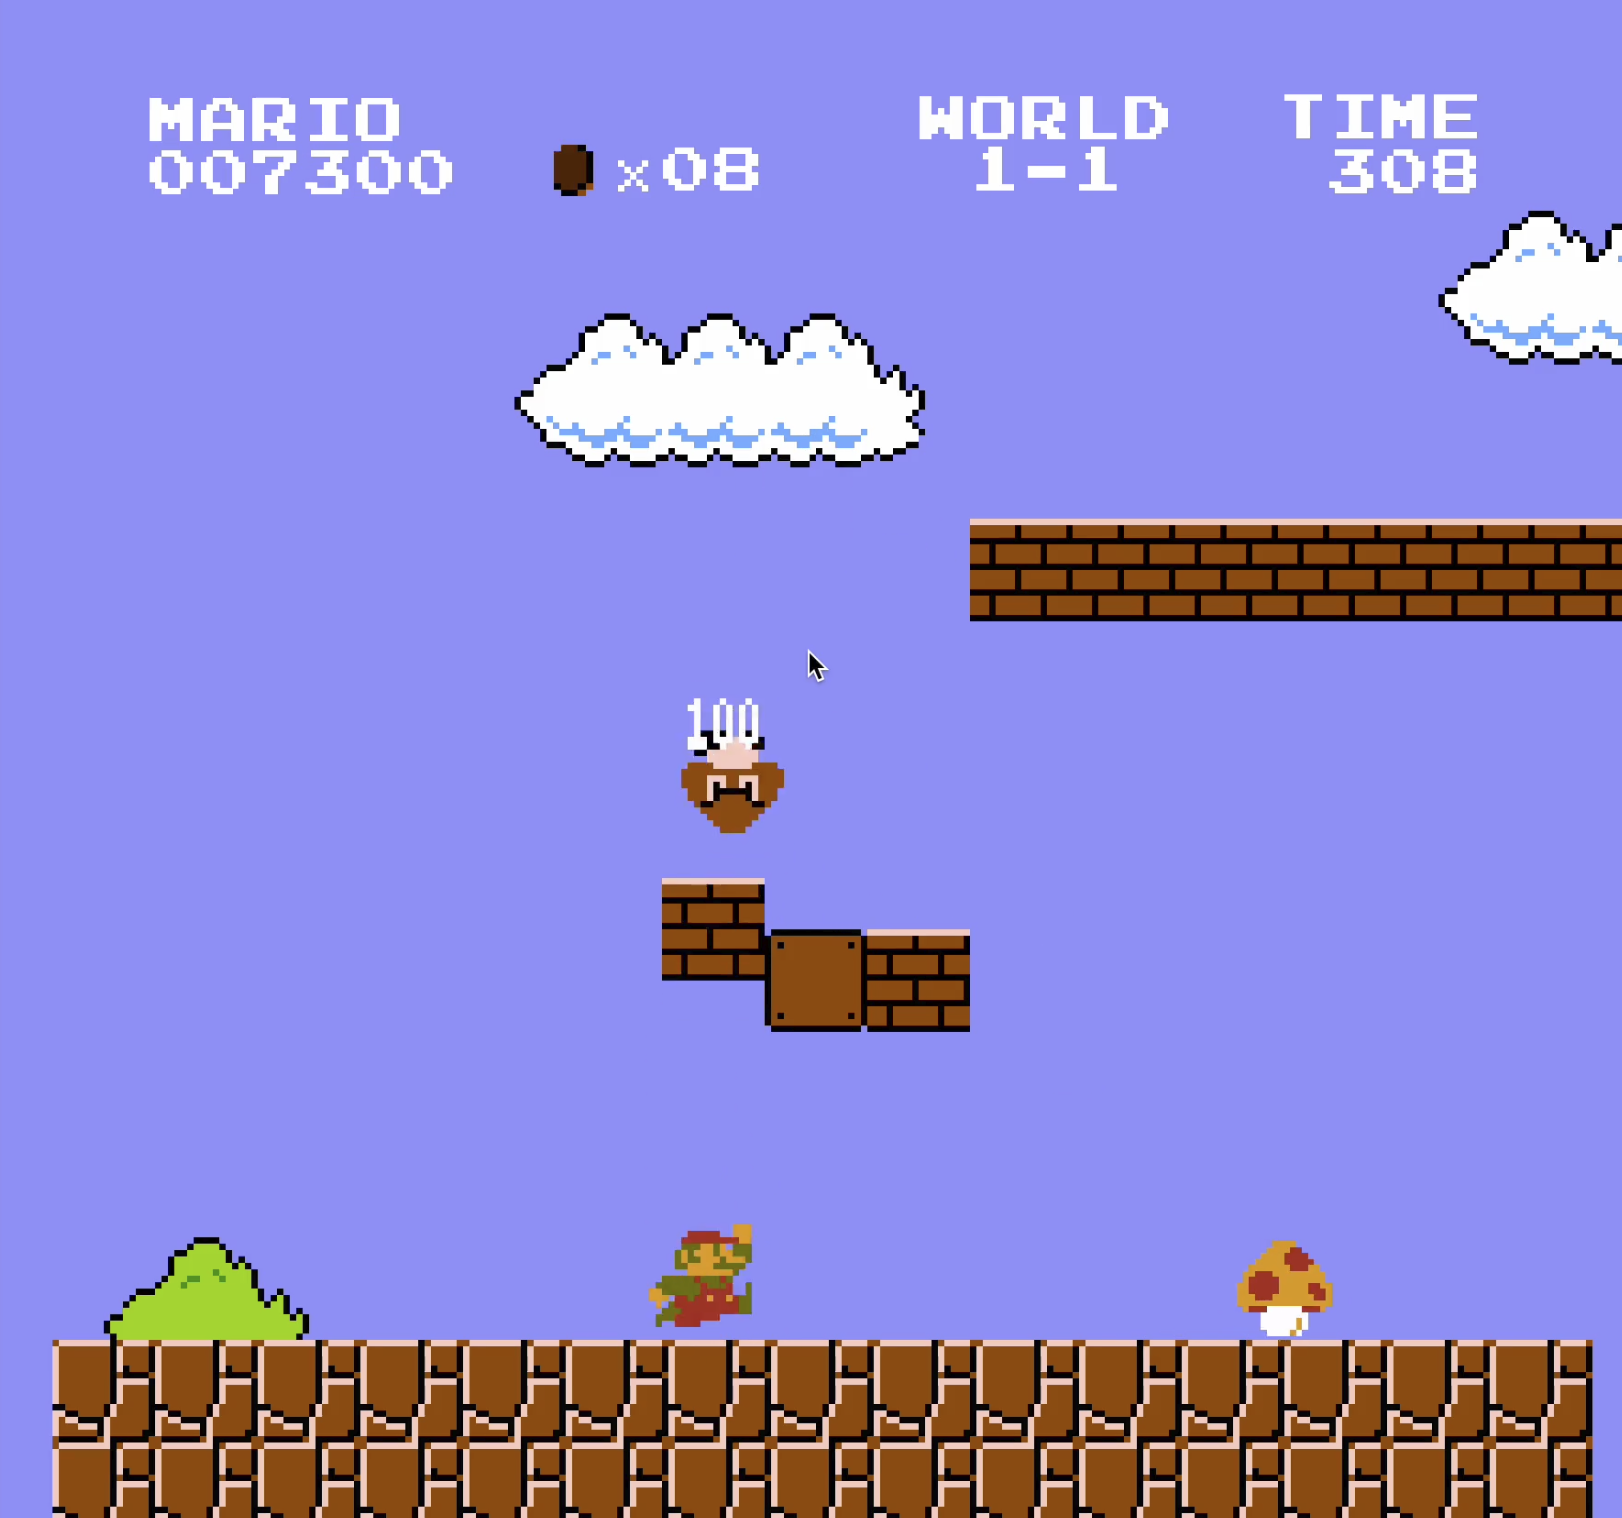
\includegraphics[width=\textwidth, height=4.6cm, keepaspectratio]{assets/in_game_2.png}
                \\[1pt]
                \scriptsize \textbf{Hình 7:} Tương tác thực thể hầm ngầm (Koopa, Brick, Mario)
            \end{tcolorbox}
            \vspace{0.05cm}
            \badge{DarkSlate}{Domain Model} \scriptsize $\ge 20$ lớp thuần C\# đáp ứng trọn vẹn nghiệp vụ.
        \end{column}
    \end{columns}
\end{frame}

% ==============================================================================
% SLIDE 9: CÁC MẪU THIẾT KẾ GoF
% ==============================================================================
\begin{frame}{Các Mẫu Thiết kế GoF (Design Patterns)}
    \begin{columns}[T]
        \begin{column}{0.50\textwidth}
            \begin{itemize}\scriptsize\setlength{\itemsep}{2pt}
                \item \textbf{1. State Pattern (Hành vi):}
                Quản lý biến hình Mario (\texttt{Small}, \texttt{Super}, \texttt{Fire}, \texttt{Dead}); loại bỏ hoàn toàn các chuỗi \texttt{if-else} / \texttt{switch} lồng nhau.

                \item \textbf{2. Factory Method Pattern (Khởi tạo):}
                \texttt{EnemyFactory} \& \texttt{ItemFactory} sinh đối tượng từ JSON schema; sẵn sàng mở rộng OCP (thêm quái mới không sửa code cũ).

                \item \textbf{3. Observer Pattern (Hành vi):}
                Sự kiện \texttt{OnScoreChanged}, \texttt{OnHealthChanged}; ngắt phụ thuộc trực tiếp giữa Core với UI Canvas và Audio.

                \item \textbf{4. Command Pattern \& DIP (Hành vi / Cấu trúc):}
                Đóng gói thao tác qua \texttt{IInputProvider}: \texttt{MoveCommand}, \texttt{JumpCommand}.

                \item \textbf{5. Object Pool Pattern (Khởi tạo):}
                Tái sử dụng \texttt{Fireball} và Particle FX; loại trừ Garbage Collection Spike (ổn định 60 FPS).
            \end{itemize}
        \end{column}

        \begin{column}{0.47\textwidth}
            \begin{tcolorbox}[colback=white, colframe=BorderGray, boxrule=0.8pt, top=2pt, bottom=2pt, left=2pt, right=2pt]
                \centering
                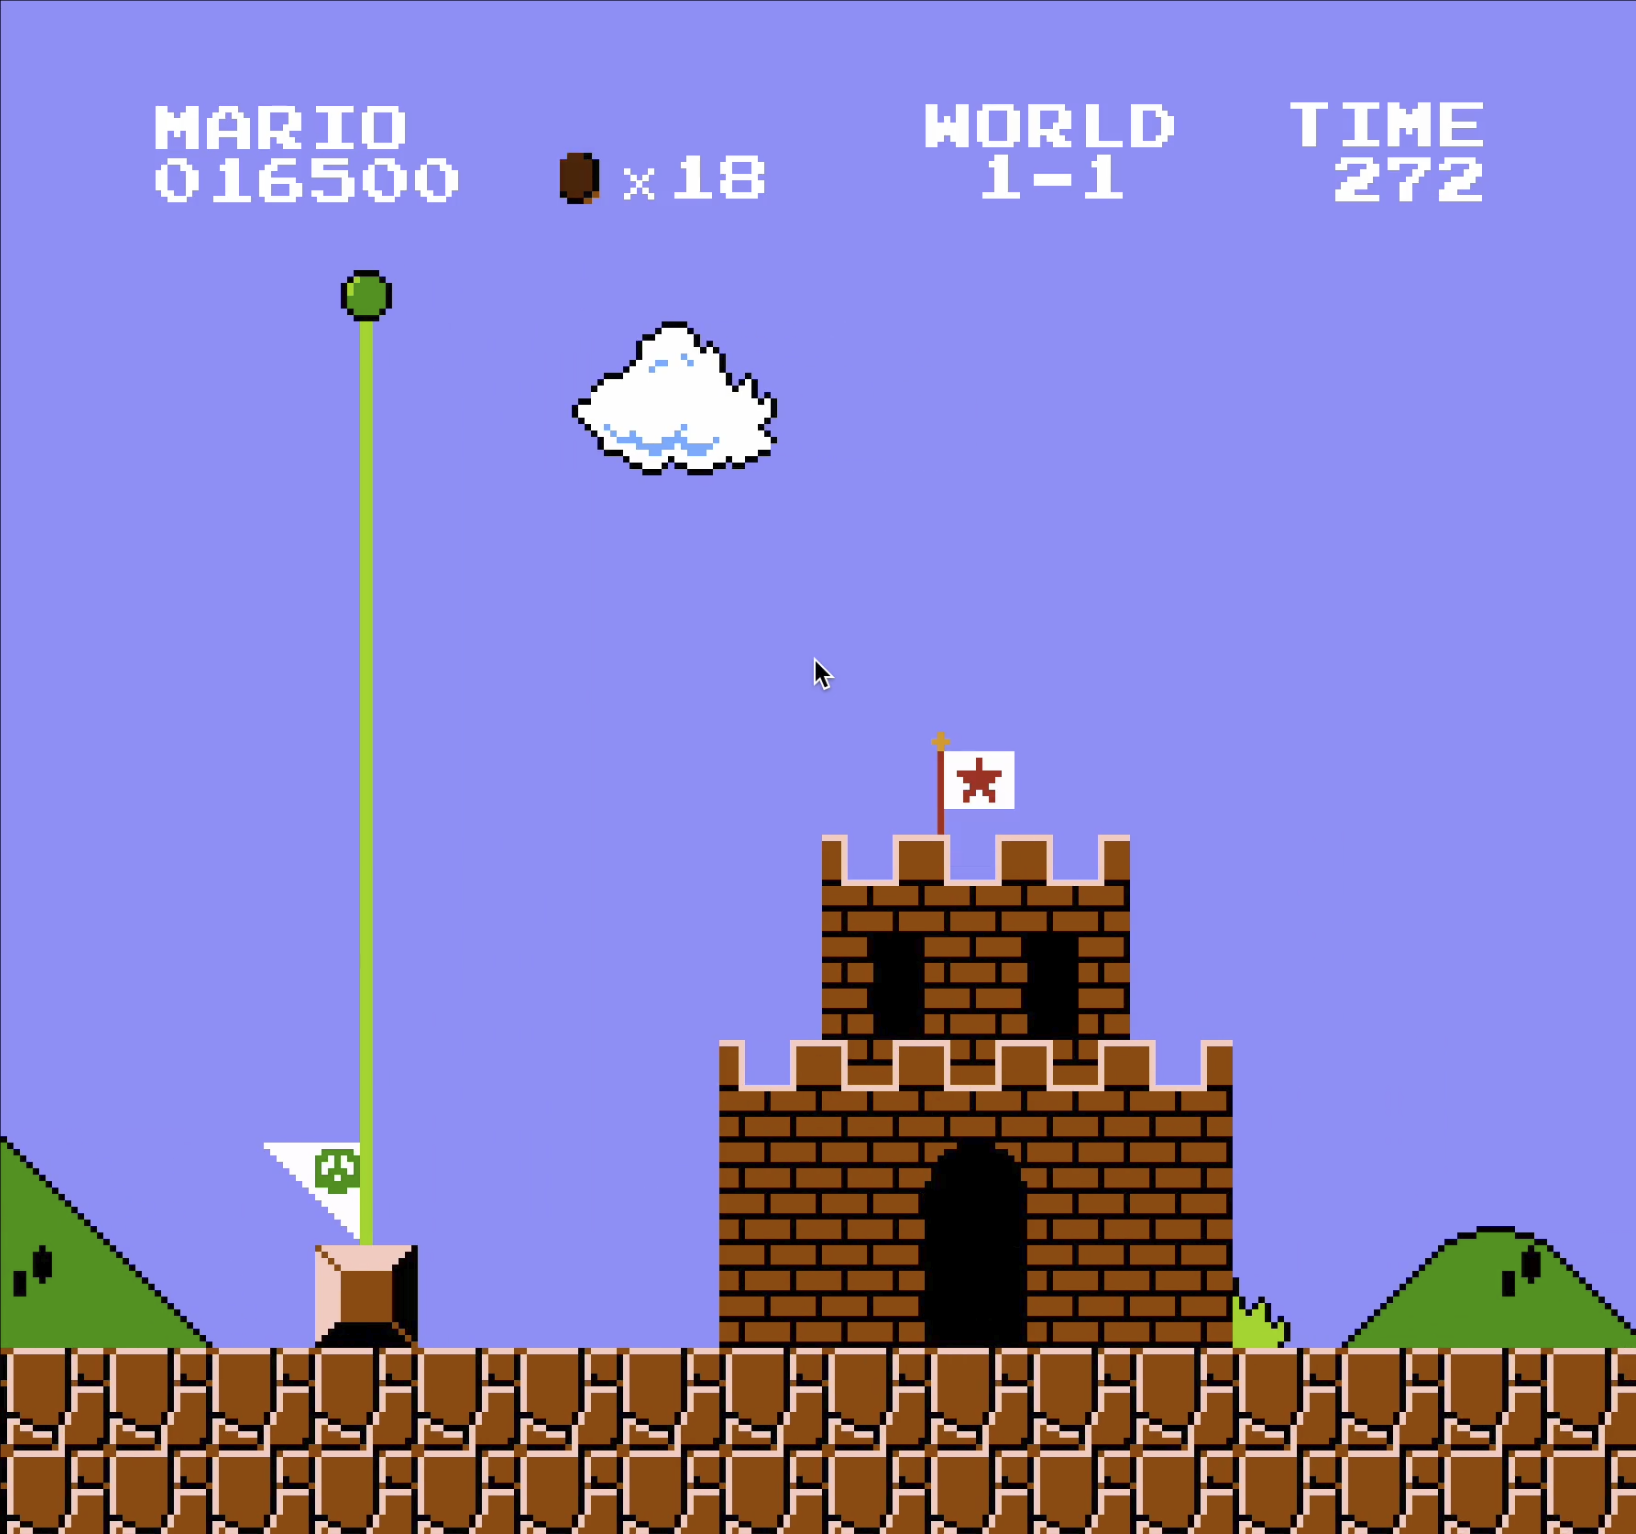
\includegraphics[width=\textwidth, height=4.6cm, keepaspectratio]{assets/in_game_3.png}
                \\[1pt]
                \scriptsize \textbf{Hình 8:} Mario bắn Fireball (State + Object Pool)
            \end{tcolorbox}
            \vspace{0.05cm}
            \badge{MarioBlue}{Đa dạng Mẫu} \scriptsize Đủ 3 nhóm GoF: Creational + Structural + Behavioral.
        \end{column}
    \end{columns}
\end{frame}

% ==============================================================================
% SLIDE 10: KIỂM THỬ PHẦN MỀM & ĐẢM BẢO CHẤT LƯỢNG (QA)
% ==============================================================================
\begin{frame}{Kiểm thử Phần mềm \& Đảm bảo Chất lượng (QA)}
    \begin{columns}[T]
        \begin{column}{0.50\textwidth}
            \textbf{\footnotesize \textcolor{HUSTRed}{Ma trận Unit Tests Pure Logic ($\ge 18$ Ca Test AAA)}}
            \begin{itemize}\scriptsize\setlength{\itemsep}{1.2pt}
                \item \textbf{TV1 (9 Tests Core):} Mario FSM, AABB overlap, Invariant 100 Coin, Save/Load snapshot.
                \item \textbf{TV2 (9 Tests Systems):} Enemy AI ledge turn, Koopa shell velocity, Factory Spawner, Object Pool recycle, Timeout GameOver.
                \item \textbf{Hiệu năng:} \textbf{100\% Tests Xanh} chạy độc lập trên CLI trong thời gian \textbf{$< 1.0$ giây}.
            \end{itemize}

            \vspace{-0.1cm}
            \textbf{\footnotesize \textcolor{MarioBlue}{Integration Tests \& Bug Log Thực tế ($\ge 6$ Bugs đã trừ khử)}}
            \begin{itemize}\scriptsize\setlength{\itemsep}{1pt}
                \item \textbf{BUG-01 (AABB Snag):} Kẹt góc tường $\rightarrow$ Sửa offset bounding box.
                \item \textbf{BUG-02 (Koopa Shell):} Mai dội ngược frame 1 $\rightarrow$ Thêm invul delay.
                \item \textbf{BUG-03 (Object Pool):} NullReference despawn $\rightarrow$ Ràng buộc unsub event.
                \item \textbf{BUG-04 (Save Corrupt):} Sai cấu trúc JSON $\rightarrow$ Bắt \texttt{SaveCorruptedException}.
            \end{itemize}
        \end{column}

        \begin{column}{0.47\textwidth}
            \begin{tcolorbox}[colback=white, colframe=BorderGray, boxrule=0.8pt, top=2pt, bottom=2pt, left=2pt, right=2pt]
                \centering
                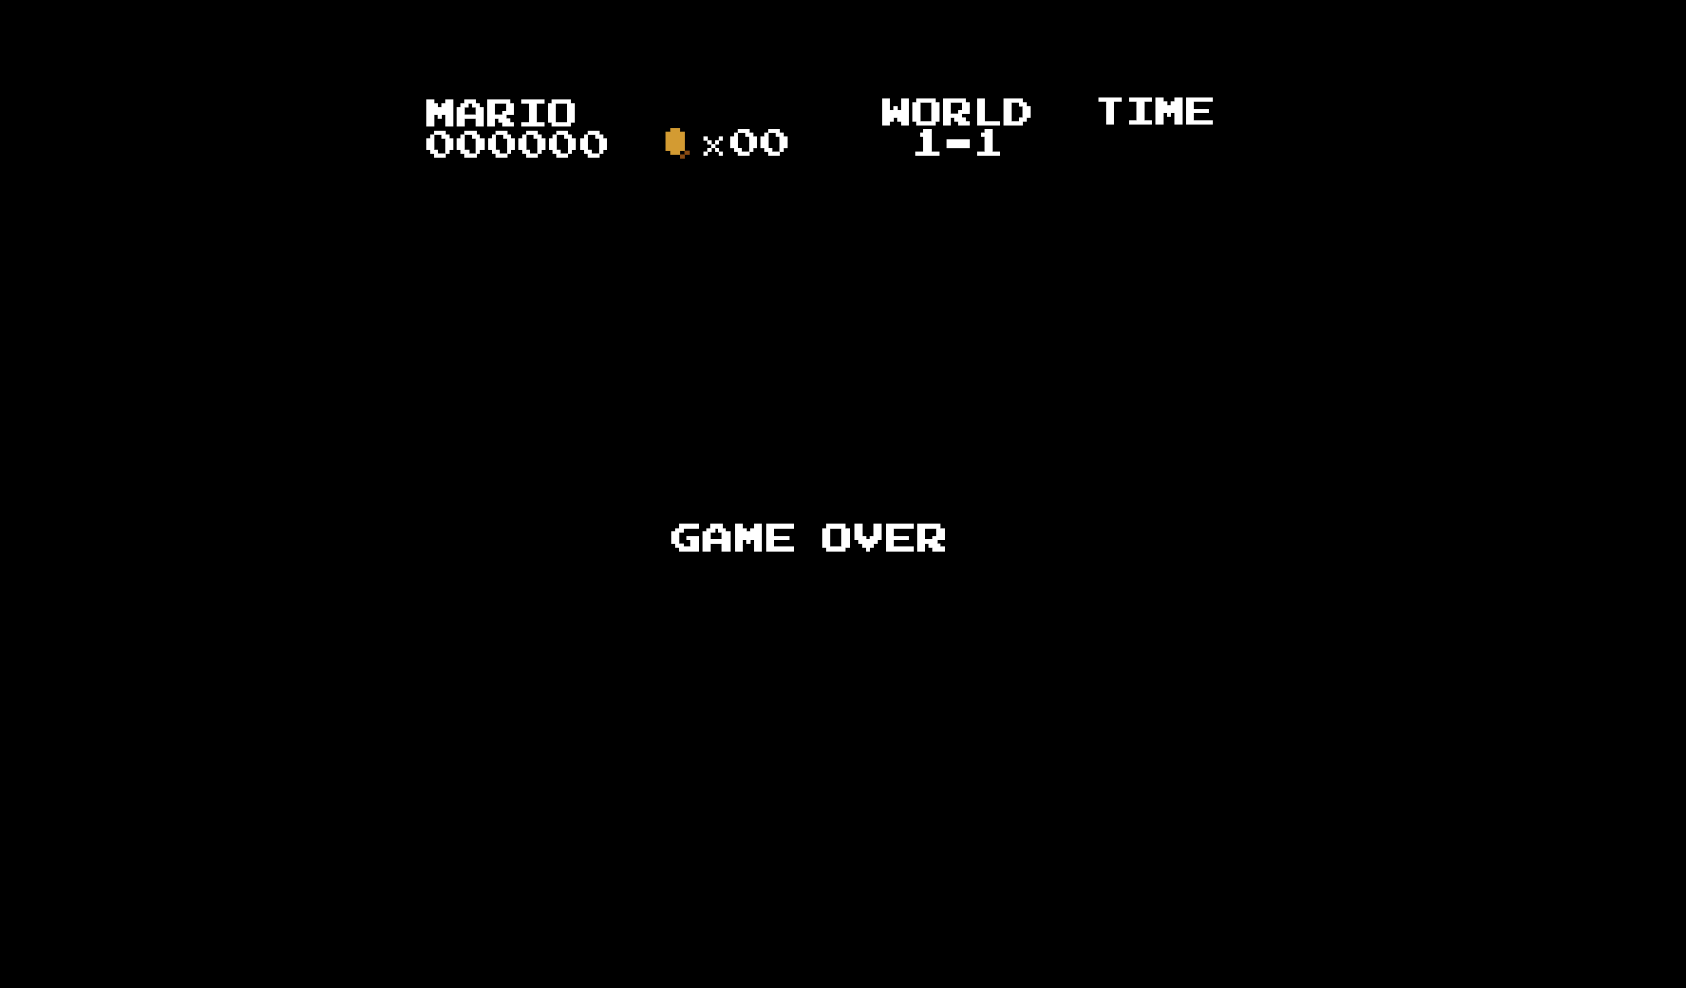
\includegraphics[width=\textwidth, height=4.6cm, keepaspectratio]{assets/game_over.png}
                \\[1pt]
                \scriptsize \textbf{Hình 9:} Màn hình Game Over khi hết mạng / Timeout
            \end{tcolorbox}
            \vspace{0.05cm}
            \badge{MarioGreen}{CI/CD Sẵn sàng} \scriptsize 100\% Pass độc lập không mở Scene Unity.
        \end{column}
    \end{columns}
\end{frame}

% ==============================================================================
% SLIDE 11: QUY CHUẨN MÃ NGUỒN & NAMING CONVENTION
% ==============================================================================
\begin{frame}{Quy chuẩn Mã nguồn \& Naming Convention}
    \begin{columns}[T]
        \begin{column}{0.50\textwidth}
            \begin{infoCard}[top=2pt, bottom=2pt]{1. Quy ước Đặt tên (Naming Conventions)}
                \begin{itemize}\scriptsize\setlength{\itemsep}{0.8pt}
                    \item \textbf{PascalCase:} Class, Struct, Enum, Method, Property. \\
                    \textit{Ví dụ:} \texttt{PlayerController}, \texttt{MarioRuleEngine}.
                    \item \textbf{\_camelCase:} Biến trường thành viên (\texttt{private fields}). \\
                    \textit{Ví dụ:} \texttt{\_moveSpeed}, \texttt{\_currentScore}.
                    \item \textbf{Tiền tố I + PascalCase:} Định danh tất cả các Interface. \\
                    \textit{Ví dụ:} \texttt{IInputProvider}, \texttt{ISaveStorage}.
                \end{itemize}
            \end{infoCard}

            \begin{successCard}[top=2pt, bottom=2pt]{2. Tiêu chuẩn Clean Code \& Tối ưu Hệ thống}
                \begin{itemize}\scriptsize\setlength{\itemsep}{0.8pt}
                    \item \textbf{0 Dead Code:} Xóa sạch script rác, file crash, thư mục thừa.
                    \item \textbf{Zero Hard-coded Paths:} 100\% dùng đường dẫn tương đối.
                    \item \textbf{SRP Tuyệt đối:} Mỗi lớp đảm nhiệm duy nhất một chức năng nghiệp vụ.
                \end{itemize}
            \end{successCard}
        \end{column}

        \begin{column}{0.47\textwidth}
            \begin{tcolorbox}[colback=white, colframe=BorderGray, boxrule=0.8pt, top=2pt, bottom=2pt, left=2pt, right=2pt]
                \centering
                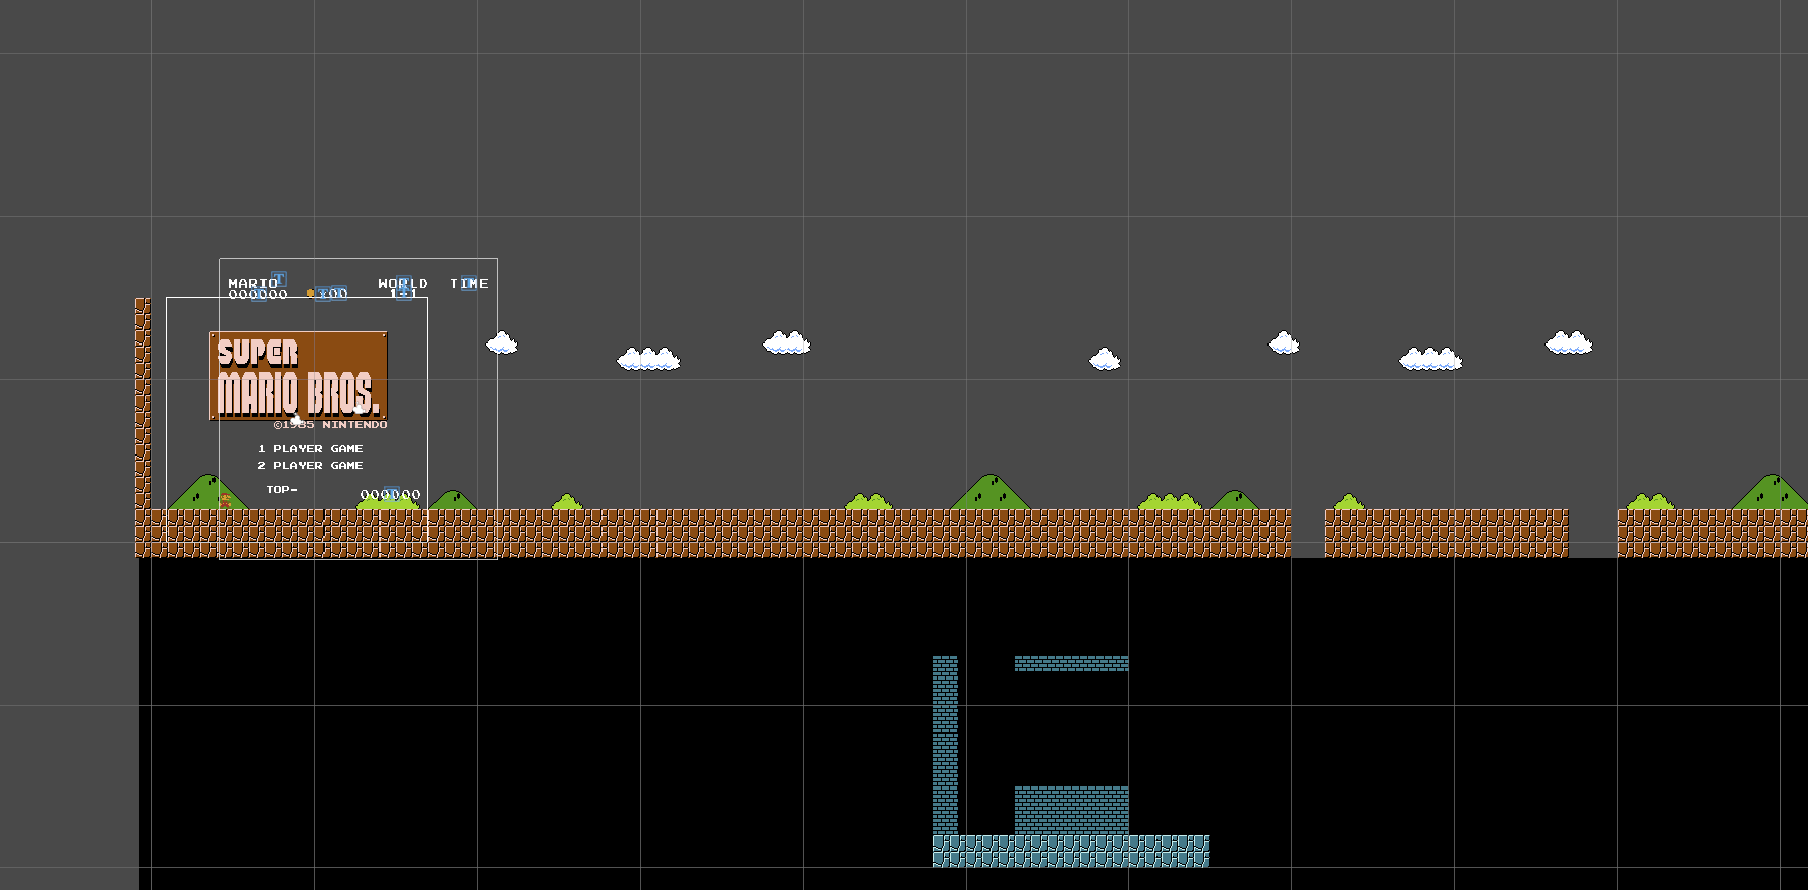
\includegraphics[width=\textwidth, height=4.2cm, keepaspectratio]{assets/edit_1.png}
                \\[1pt]
                \scriptsize \textbf{Hình 10:} Cấu trúc thư mục mã nguồn chuẩn hóa
            \end{tcolorbox}
            \vspace{0.04cm}
            \badge{DarkSlate}{Kiểm toán Tĩnh} \scriptsize 0 Cảnh báo lỗi nghiêm trọng trong IDE.
        \end{column}
    \end{columns}
\end{frame}

% ==============================================================================
% SLIDE 12: TỔNG KẾT & KIỂM ĐỊNH HAI CHIỀU A <-> B
% ==============================================================================
\begin{frame}{Tổng kết \& Sẵn sàng Vấn đáp Live Audit}
    \begin{columns}[T]
        \begin{column}{0.50\textwidth}
            \begin{coreCard}[top=2pt, bottom=2pt]{Đánh giá Tổng thể theo Khung 2 Trục}
                \begin{itemize}\scriptsize\setlength{\itemsep}{1pt}
                    \item \textbf{Trục I (Hoàn thiện Sản phẩm):} Đạt trần \textbf{4.00 / 4.00 điểm} (40\%) \\
                    5 màn + 2 chế độ, Save/Load JSON 100\%, Clean-Room build $\le 3$ phút.
                    \item \textbf{Trục II (Độ hiểu sâu Thiết kế -- Mã nguồn):} Đạt trần \textbf{6.00 / 6.00 điểm} (60\%) \\
                    Kiến trúc 3 tầng sạch, 18 Unit Tests AAA, 5 Design Patterns, khớp $A \leftrightarrow B$.
                \end{itemize}
            \end{coreCard}

            \begin{successCard}[top=2pt, bottom=2pt]{Sẵn sàng Diễn tập Vấn đáp Sống (Live Defense Probes)}
                \begin{itemize}\scriptsize\setlength{\itemsep}{1pt}
                    \item \textbf{Live OCP Probe (2--3 phút):} Thêm quái mới (\textit{Hammer Bro}) không sửa mã nguồn cũ bằng Registry / Factory.
                    \item \textbf{Live Fault-Injection:} Tiêm lỗi điều kiện sống và dùng Debugger (Call Stack, Watch) định vị và sửa trực tiếp.
                \end{itemize}
            \end{successCard}
        \end{column}

        \begin{column}{0.47\textwidth}
            \begin{tcolorbox}[colback=white, colframe=BorderGray, boxrule=0.8pt, top=2pt, bottom=2pt, left=2pt, right=2pt]
                \centering
                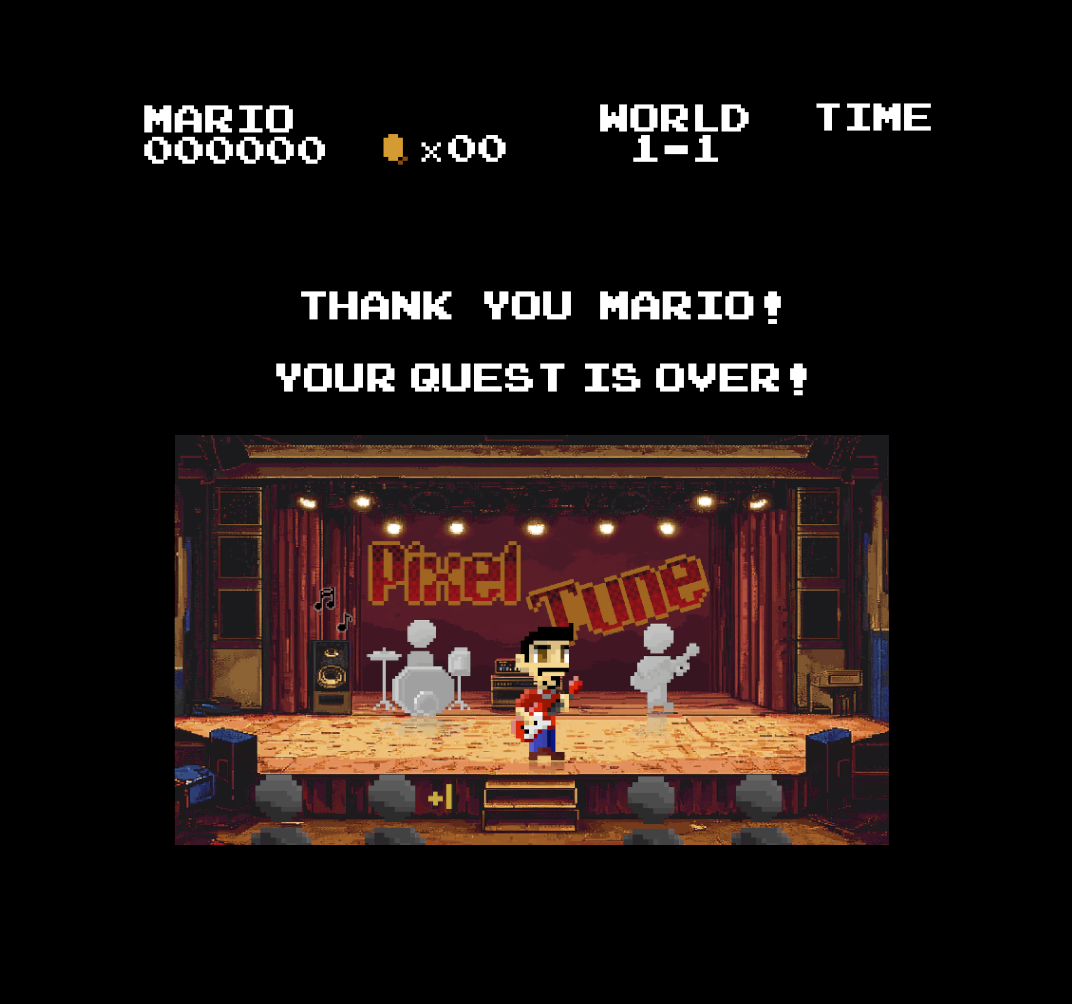
\includegraphics[width=\textwidth, height=3.8cm, keepaspectratio]{assets/win_game.png}
                \\[1pt]
                \scriptsize \textbf{Hình 11:} Mario chạm cờ chiến thắng kết thúc màn chơi
            \end{tcolorbox}
        \end{column}
    \end{columns}
\end{frame}

\end{document}
